\section{圆的初步}
\subsection{四点共圆的判定}
四点共圆的条件:四点A,B,C,D共圆的充要条件为:$\angle{ABC}=\angle{ADC}\neq0$(同侧)
或$\angle{ABC}+\angle{ADC}=180^{\circ}$(异侧).

此外,相交弦定理逆定理,切割线定理逆定理,托勒密定理逆定理等许多关于圆的相关定理的逆定理
也都可作为四点共圆的判据,需要根据题目条件灵活使用(不过使用做多的还是利用角度进行判断)。

四点共圆在平几题中出现频率非常高,在问题中一般有两种形式:一是作为证题的目的;通常需要根据
题设条件推出判定四点共圆的条件(前述的几种),也可以用两组四点共圆来证明题设要求的四点共圆;
二是作为解题的工具,可以用于证明角相等、线垂直等。
\begin{figure}[H]
    \centering  
    \subfigure{
    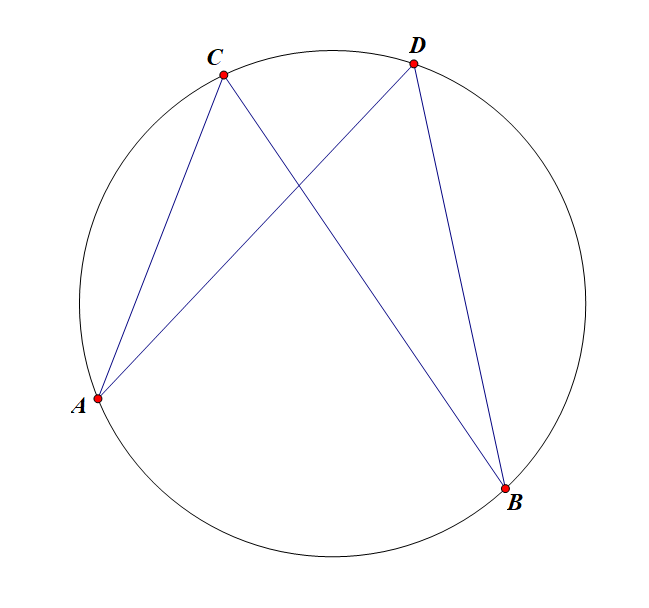
\includegraphics[scale=0.4]{4}}
    \subfigure{
    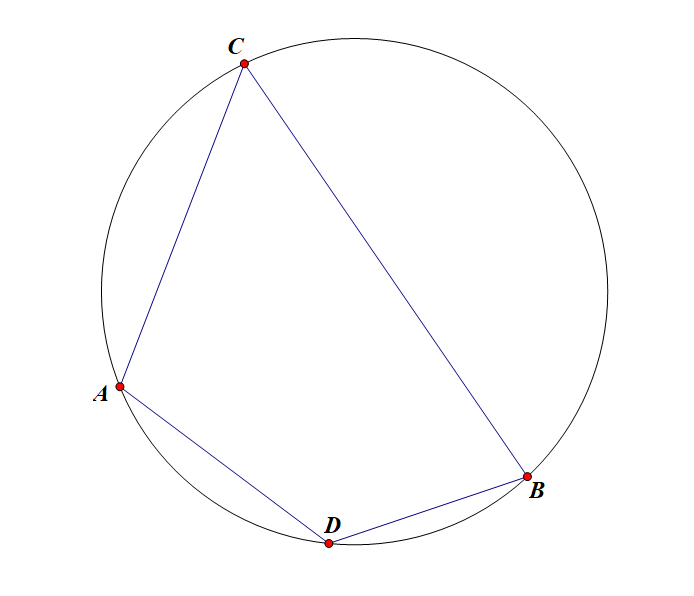
\includegraphics[scale=0.4]{5}}
\end{figure}
\subsection{与圆相关的定理}
(1)托勒密定理:在凸四边形ABCD中,$AB\cdot CD+AD\cdot BC\geq AC\cdot BD$,
当且仅当四边形ABCD是圆内接四边形时,等号成立。
\begin{center}
    \includegraphics*[scale=0.5]{1.png}
\end{center}

三弦定理:设PA,PB,PC是圆内一公共端点的三条弦,则
$$PA\sin{\angle{BPC}}+PC\sin{\angle{APB}}=PB\sin{\angle{APC}}$$

三弦定理逆定理:设PA,PB,PC是一公共端点的三条线段,若
$$PA\sin{\angle{BPC}}+PC\sin{\angle{APB}}=PB\sin{\angle{APC}}$$
则P,A,B,C四点共圆。
\begin{center}
    \includegraphics*[scale=0.3]{2.png}
\end{center}

(2)西姆松定理
过三角形外接圆上异于三角形顶点的任意一点作三边的垂线,则三垂足点共线(此线称为西姆松线)。
\begin{center}
    \includegraphics*[scale=0.5]{3.png}
\end{center}

(3)帕斯卡定理
圆内接六边形ABCDEF三组对边(延长线)的交点P、Q、R三点共线。
\begin{figure}[H]
    \centering  
    \subfigure{
    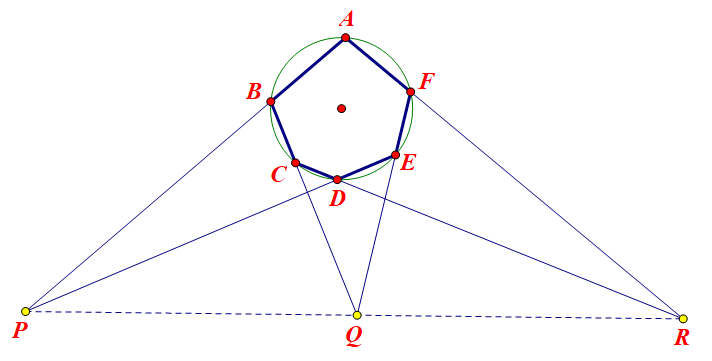
\includegraphics[scale=0.5]{6}}
    \subfigure{
    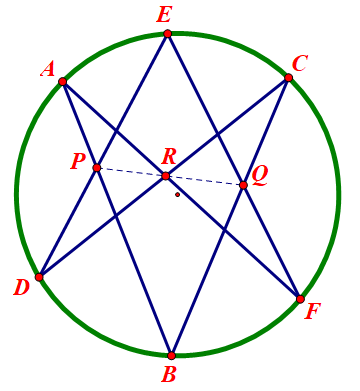
\includegraphics[scale=0.5]{7}}
\end{figure}
\newpage
\subsection{例题}
1.$\quad$ AB是圆O的直径.C与D是互异的圆O上的两点,且在AB的一侧.过C、D作圆的切线交于点E.线段AD与BC交于点F,直线EF交AB于M.求证:E,C,M,D四点共圆.
\begin{center}
    \includegraphics*[scale=0.4]{20}
\end{center}

~\\
~\\
~\\
~\\
~\\
~\\

2.A、B、C三点共线,O点在直线外。$O_1,O_2,O_3$分别
为$\bigtriangleup OAB,\bigtriangleup OBC,\bigtriangleup OCA$的外心.求证: 
$O,O_1,O_2,O_3$四点共圆.
\begin{center}
    \includegraphics*[scale=0.4]{21}
\end{center}
\newpage

3.$\bigtriangleup ABC$中,$AB=AC$,点E,F分别在AB,AC上,$AE<AF$,BF,CE交于点P.求证:$PF<PE$.
\begin{center}
    \includegraphics*[scale=0.4]{22}
\end{center}

~\\

4.圆O过$\bigtriangleup ABC$顶点A、C,且与AB、BC交于K、N(K、N不同).$\bigtriangleup ABC$外接圆和$\bigtriangleup BKN$外接圆交于B、M两点。求证:
$\angle{BMO}=90^{\circ}$.
\begin{center}
    \includegraphics*[scale=0.4]{23}
\end{center}


5.在平行四边形ABCD中,过点C作AB,AD的垂线CM,CN,垂足分别为M,N,MN,BD的延长线交于点P.求证:PC$\bot $AC.
\begin{center}
    \includegraphics*[scale=0.4]{24}
\end{center}

